\begin{figure}[!htb]
    \begin{center}
    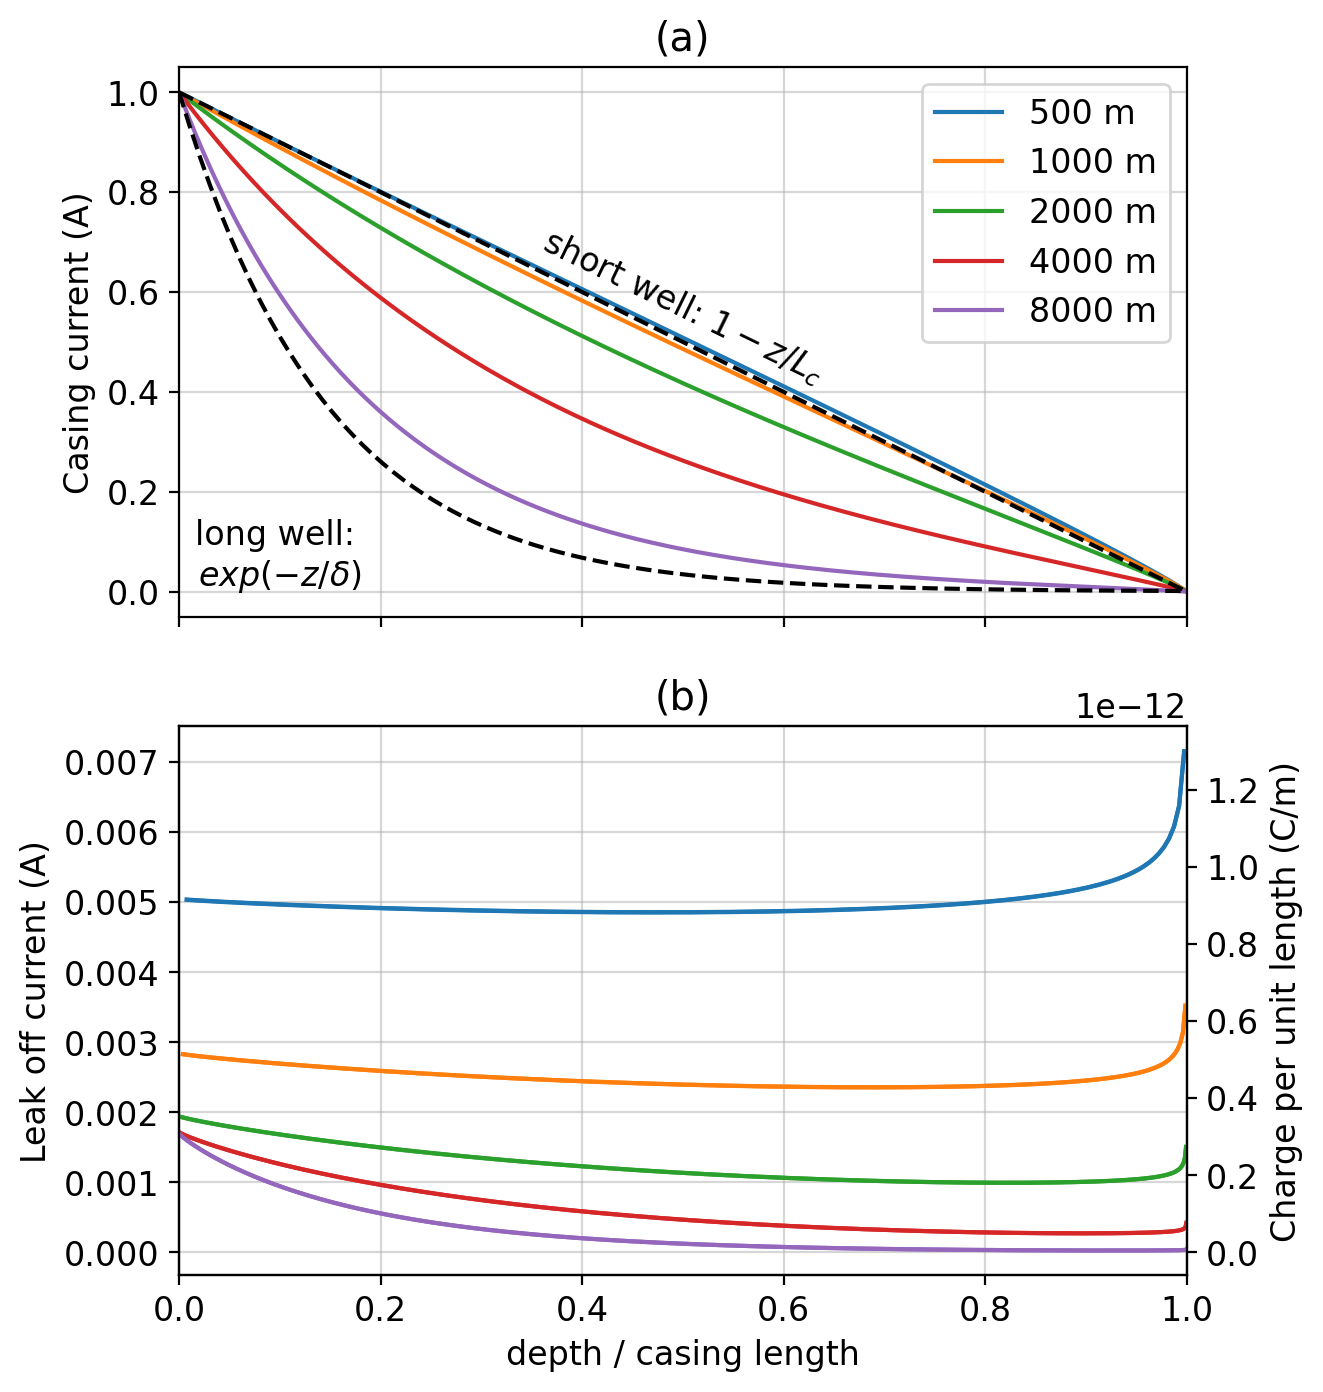
\includegraphics[width=0.55\textwidth]{figures/finite-wells.png}
    \end{center}
\caption{
    Currents in a DC resistivity experiment with the positive electrode connected to the top of the casing.
    (a) Downward-going currents in the casing for different lengths of well. The x-axis is depth normalized by the length of the casing.
    Annotations are the short and long well approximations from \cite{Kaufman1993}. For the long-well approximation, we use $L_c = 8000m$, the length of the longest well included in the simulation.
    (b) Leak-off currents from the well (left axis) and charges on the outer casing wall (right axis).
    Figure follows \cite{Heagy2019a}.
}
\label{fig:finite-wells}
\end{figure}
